\documentclass{article}
\usepackage{amsmath}
\usepackage{amsthm}
\usepackage{amsfonts}
\usepackage{amssymb}
\usepackage{bbold}
\usepackage{dsfont}
\usepackage{graphicx}
\usepackage{cleveref}
\usepackage{bm}
\usepackage{booktabs}
\usepackage{siunitx}
\usepackage{xcolor}
\usepackage[utf8]{inputenc}
\usepackage[english]{babel}
\newtheorem{definition}{Definition}
\newtheorem{example}{Example}
\newcommand{\exP}[1]{\mathrm{e}^{#1}}
\newcommand{\dif}{\mathrm{d}}
\renewcommand{\vec}[1]{\mathbf{#1}}
\newcommand{\pdagger}{{\phantom{\dagger}}}
\newcommand{\state}[1]{\vert #1\rangle}
\newcommand{\cstate}[1]{\langle #1\vert}
\newcommand{\tr}[1]{\mathrm{tr}\left\{#1\right\}}
\newcommand{\trs}[2]{\, \mathrm{tr}_{#1}\{#2\}}
\newcommand{\expc}[3]{\langle #1\vert #2 \vert #3\rangle}
\usepackage[doi=false,url=false,isbn=false,backend=bibtex,style=nature,natbib=true,sorting=none]{biblatex}
\bibliography{bib.bib}
\usepackage{geometry}
\geometry{
	a4paper,
	total={170mm,257mm},
	left=20mm,
	top=20mm,
}
\begin{document}
	
\title{Fransson's model: Tests of implementation}
\author{Rudolf Smorka}
\maketitle
\section{Model}
The model considered for a chiral, single-stranded molecule, as proposed in Refs.~\cite{fransson2019chirality,fransson2020vibrational,Fransson_2021,fransson2021charge}, reads
\begin{align}
	\hat{H} &= \hat{H}_\mathrm{mol} + \hat{H}_\mathrm{env} + \hat{H}_\mathrm{sys-env}.
\end{align} 
The molecular Hamiltonian is modeled by a combination of the  Peierls and the Kane-Mele models. It consists of an electronic on-site, nearest-neighbor hopping, and next-to-nearest neighbor spin-orbit coupling (SOC), a Peierls electron-phonon coupling and vibrational contribution to SOC, and the harmonic phonon potential energy 
\begin{align}
	\hat{H}_\mathrm{mol} &= \hat{H}_\mathrm{el} + \hat{H}_\mathrm{el-ph} + \hat{H}_\mathrm{ph},\\
	\begin{split}
		\hat{H}_\mathrm{el} &= \sum_{j,\sigma} \varepsilon_{j\sigma}^\pdagger \hat{d}_{j\sigma}^\dagger \hat{d}_{j\sigma}^\pdagger - t_0 \sum_{j\sigma} (\hat{d}_{j\sigma}^\dagger \hat{d}_{j+1,\sigma}^\pdagger + \mathrm{h.c.}) +\\& \lambda_0^\pdagger\sum_{j\sigma\sigma'} (i\hat{d}_{j\sigma}^\dagger (\vec{v}_j^{(+)}\cdot \bm{\sigma})_{\sigma\sigma'}^\pdagger \hat{d}_{j+2,\sigma'}^\pdagger + \mathrm{h.c.}),
	\end{split}\\
	\hat{H}_\mathrm{el-ph} &= - t_1^\pdagger \sum_{j,\sigma}  \hat{d}_{j\sigma}^\dagger \hat{d}_{j+1\sigma}^\pdagger (\hat{a}_{j}^\dagger + \hat{a}_{j}^\pdagger) \\ & + \lambda_1^\pdagger\sum_{j\sigma} (i \hat{d}_{j\sigma}^\dagger (\vec{v}_j^{(+)} \cdot \bm{\sigma})_{\sigma\sigma'}^\pdagger \hat{d}_{j+2\sigma'}^\pdagger +\mathrm{h.c.})(\hat{a}_{j}^\dagger + \hat{a}_{j}^\pdagger),\label{eq:HelPh}\\
	\hat{H}_\mathrm{ph} &= \sum_{j} \omega_{j}^\pdagger \hat{a}_{j}^\dagger \hat{a}_{j}^\pdagger.
	 \label{eq:Hamiltonian_el_Fransson} 
\end{align}
This molecule is coupled to an environment of spin-full, noninteracting electrons
\begin{equation}
	H_\mathrm{env} = \sum_{\ell k\sigma} \varepsilon_{\ell k\sigma}^\pdagger c_{\ell k\sigma}^\dagger c_{\ell k\sigma}^\pdagger \label{eq:LeadHamiltonian}
\end{equation}
and the system-environment coupling is linear in the molecular and environmental operators (only at the first and last site of the molecule)
\begin{align}
	H_\mathrm{sys-env} &= \sum_{\sigma\sigma'}(\nu_{L\sigma\sigma'}^\pdagger c_{N_L\sigma}^\dagger d_{1\sigma'}^\pdagger + \nu_{R\sigma\sigma'}^\pdagger c_{1_R\sigma}^\dagger d_{\mathbb{M}\sigma'}^\pdagger + \mathrm{h.c.}). \label{eq:LeadSysHamiltonian}
\end{align} 
\section{Methods}
In the following, we compare the dynamics in the model defined above using a variety of methods. 
\begin{itemize}
	\item Exact diagonalization (ED): Valid for isolated molecule, phonons treated quantum-mechanically.
	\item Time-dependent variational principle based on a matrix-product state Ansatz (TDVP): Valid for isolated molecule, phonons treated quantum-mechanically.
	\item Hierarchical equations of motion in matrix product state representation (TT-HEOM): Valid for both isolated molecule and molecule coupled to leads, phonons treated quantum-mechanically.
	\item Hierarchical equations of motion in combination with Ehrenfest dynamics (MF-HEOM): Valid for purely electronic dynamics in both isolated molecule and molecule coupled to leads. Phonons approximated to be classical.
\end{itemize}
\newpage
\section{Comparison of Dynamics in Isolated Molecule}
\subsection{On-site and Hopping}
Parameters: $L=3$, $t_0 = 1$, $\varepsilon_\uparrow = 1= -\varepsilon_\downarrow$. All methods agree nearly perfectly with each other. Within the TT-HEOM approach (here the bond dimension is $r=100$), it has been checked that the deviation of the norm of the state from unity $1-\vert \vert\rho\rangle\vert $ remains below $10^{-8}$ for the entire time interval considered here.
\begin{figure}[!h]
	\centering
	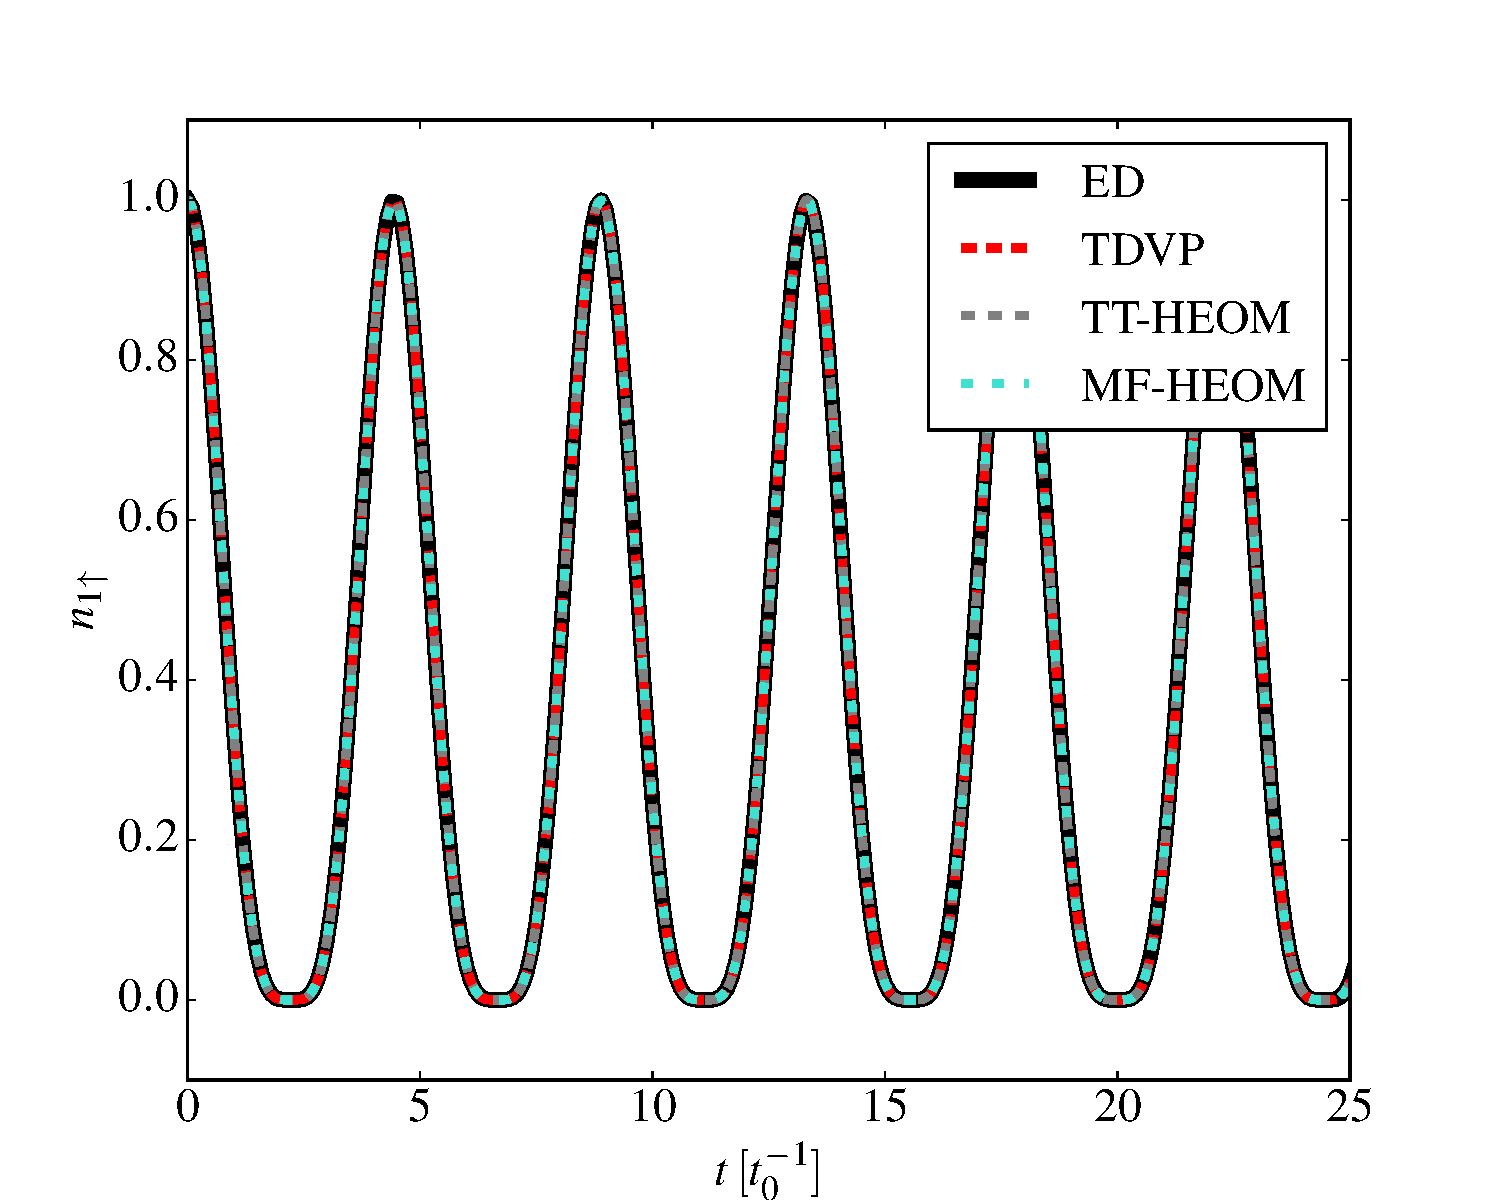
\includegraphics[width=0.72\textwidth]{figs/Comparison_TTHEOM_MFHEOM_TDVP_ED_hop+onsite.pdf}
\end{figure}
\subsection{On-site, Hopping, and SOC}
Parameters: $L=3$, $t_0 = 1$, $\varepsilon_\uparrow = 1= -\varepsilon_\downarrow$, $\lambda = 0.8$. Similar as above, the deviation of the norm from unity is the same.
\begin{figure}[!h]
	\centering
	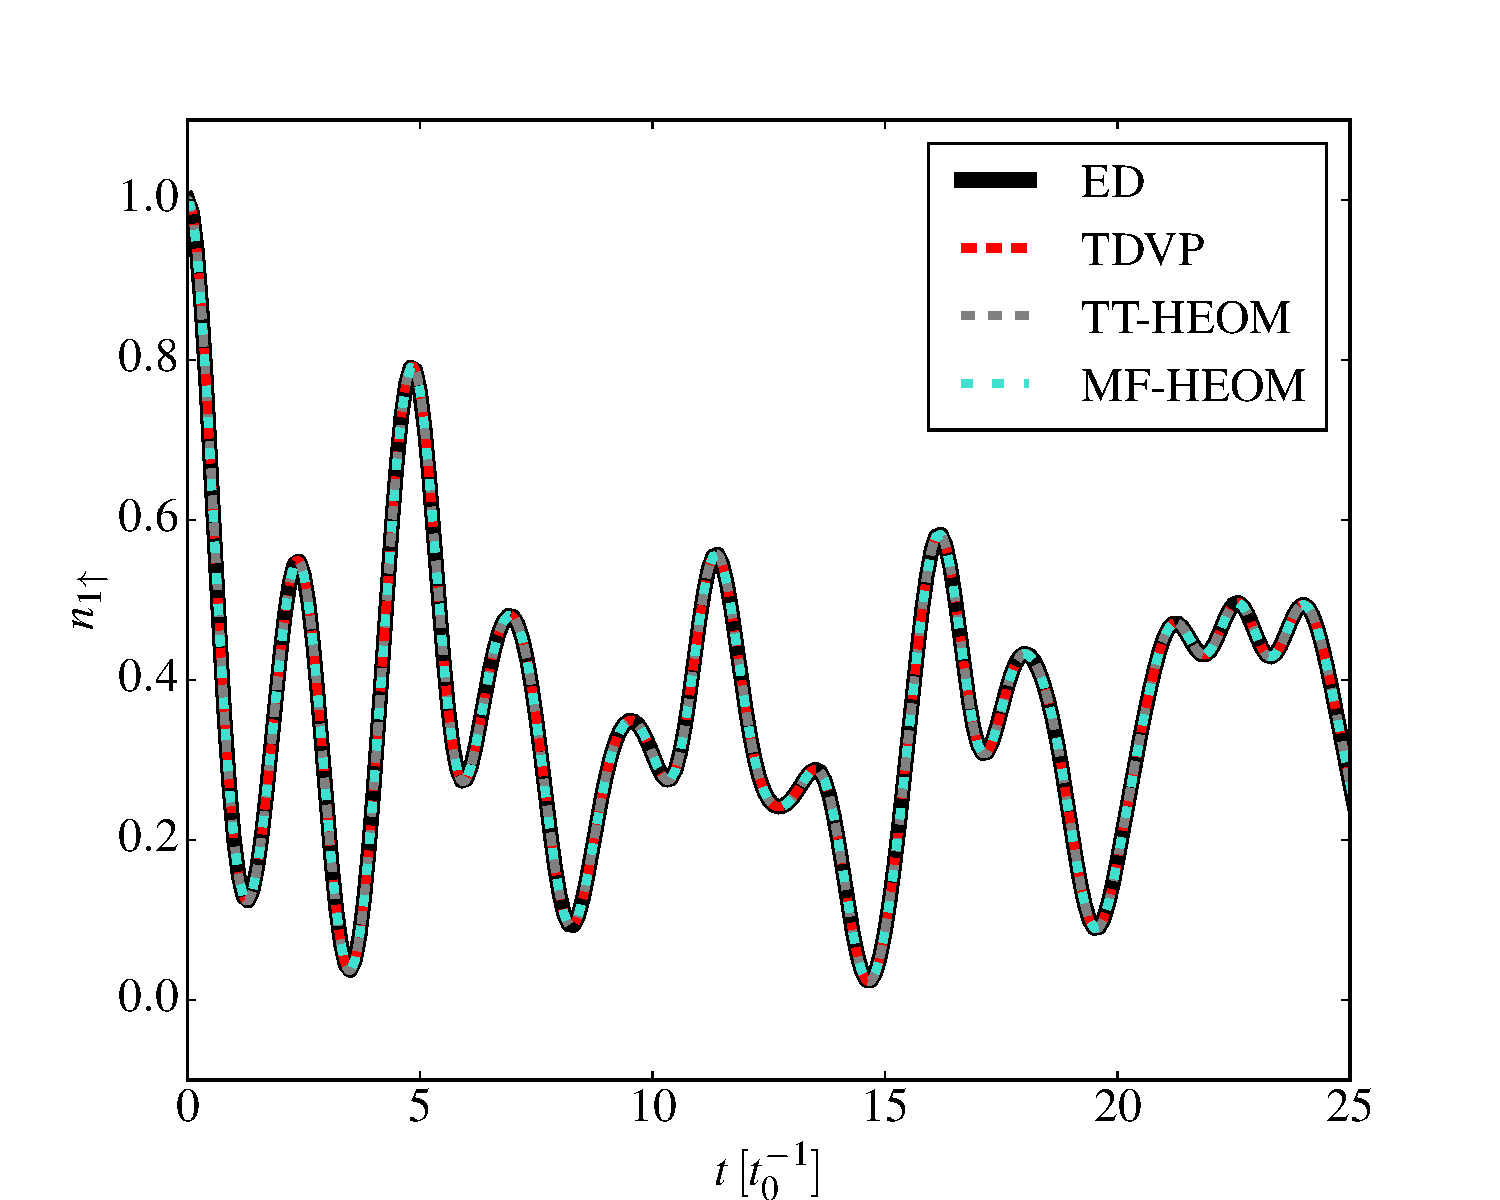
\includegraphics[width=0.72\textwidth]{figs/Comparison_TTHEOM_MFHEOM_TDVP_ED_hop+onsite+soc.pdf}
\end{figure}
\subsection{Hopping and Peierls distortion}
Parameters: $L=3$, $t_0 = 1$, $t_1 = 0.1t_0$. The ED has been checked to be converged; for the time interval considered here, 5 number of states per vibrational mode are sufficient for convergence. The TT-HEOM method agrees with ED and TDVP only for very short times; for $t\geq 8$, the TT-HEOM results deviate the norm drops down significantly. Increasing the rank from $r=100$ to $r=150$ leads to slightly better behavior of the norm. The overall population dynamics, however, changes only slightly. 
\begin{figure}[!h]
	\centering
	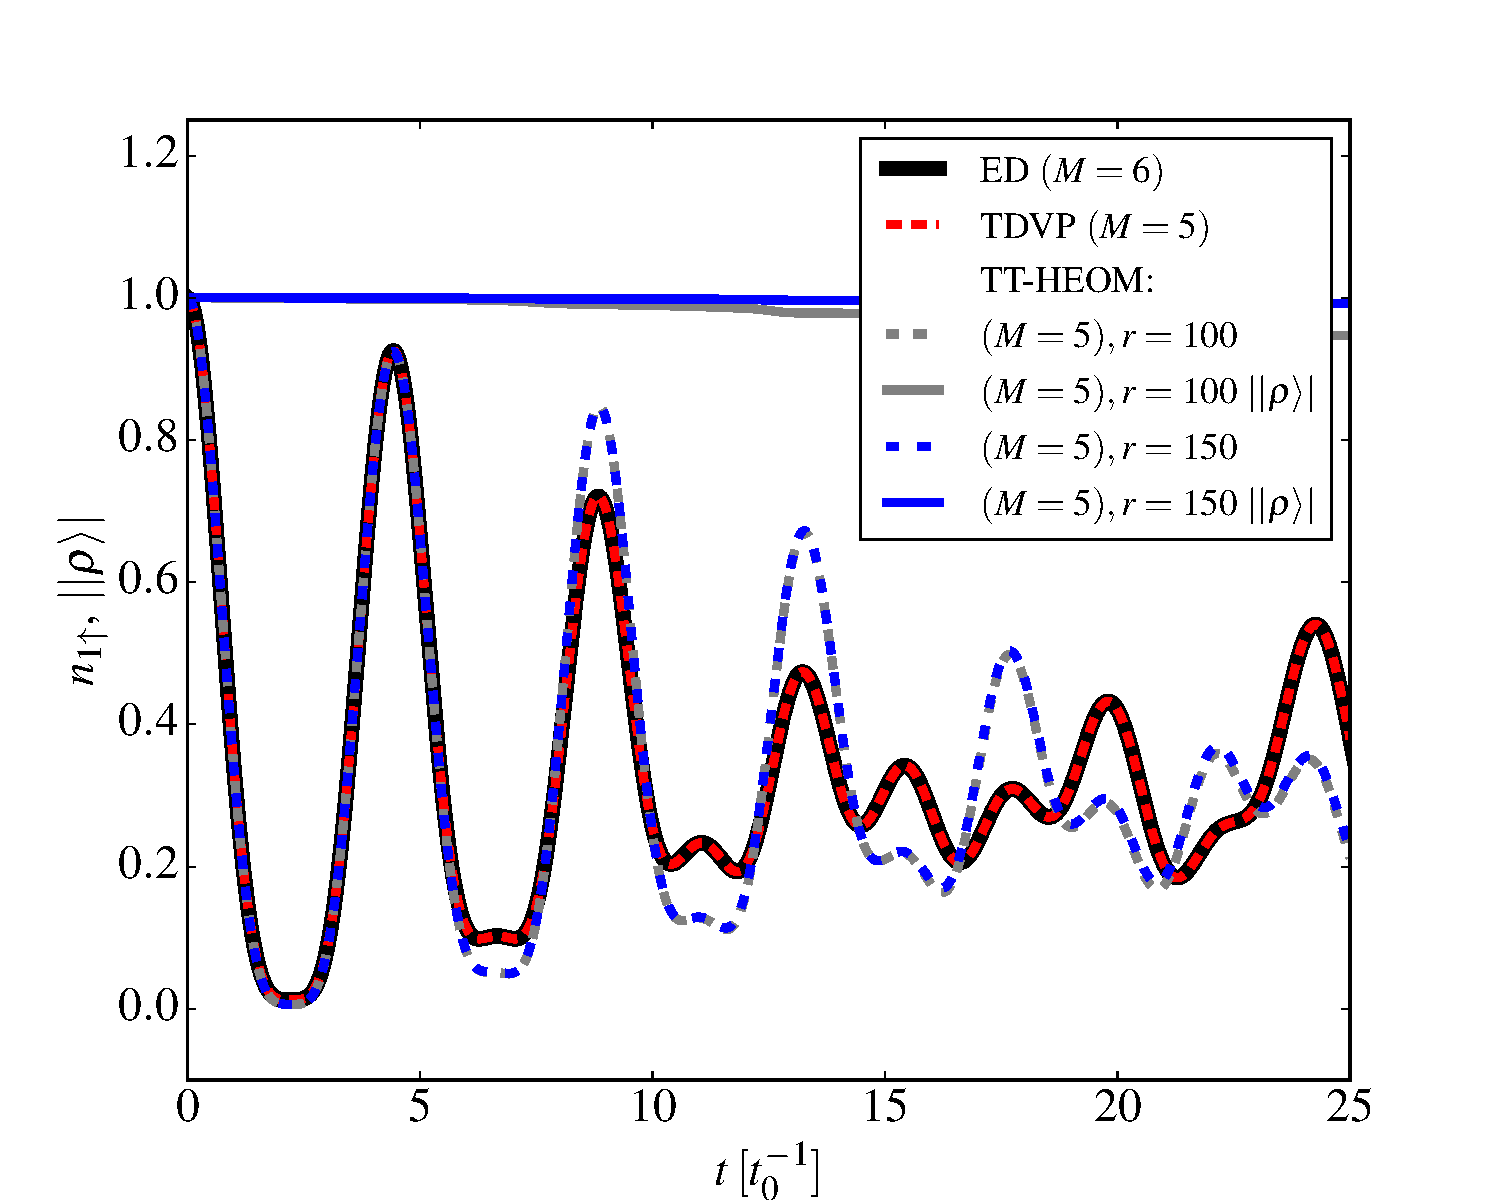
\includegraphics[width=0.705\textwidth]{figs/Comparison_TTHEOM_TDVP_ED_hop+onsite+tph.pdf}
\end{figure}
\subsection{Hopping, SOC, and Peierls distortion}
Parameters: $L=3$, $t_0 = 1$, $\lambda_0 = t_0/40$, $t_1 = 0.1t_0$. As $t_1$ dominates the dynamics, the results remains essentially unchanged in comparison to the case above. Hence, convergence issues in the TT-HEOM remain.
\begin{figure}[!h]
	\centering
	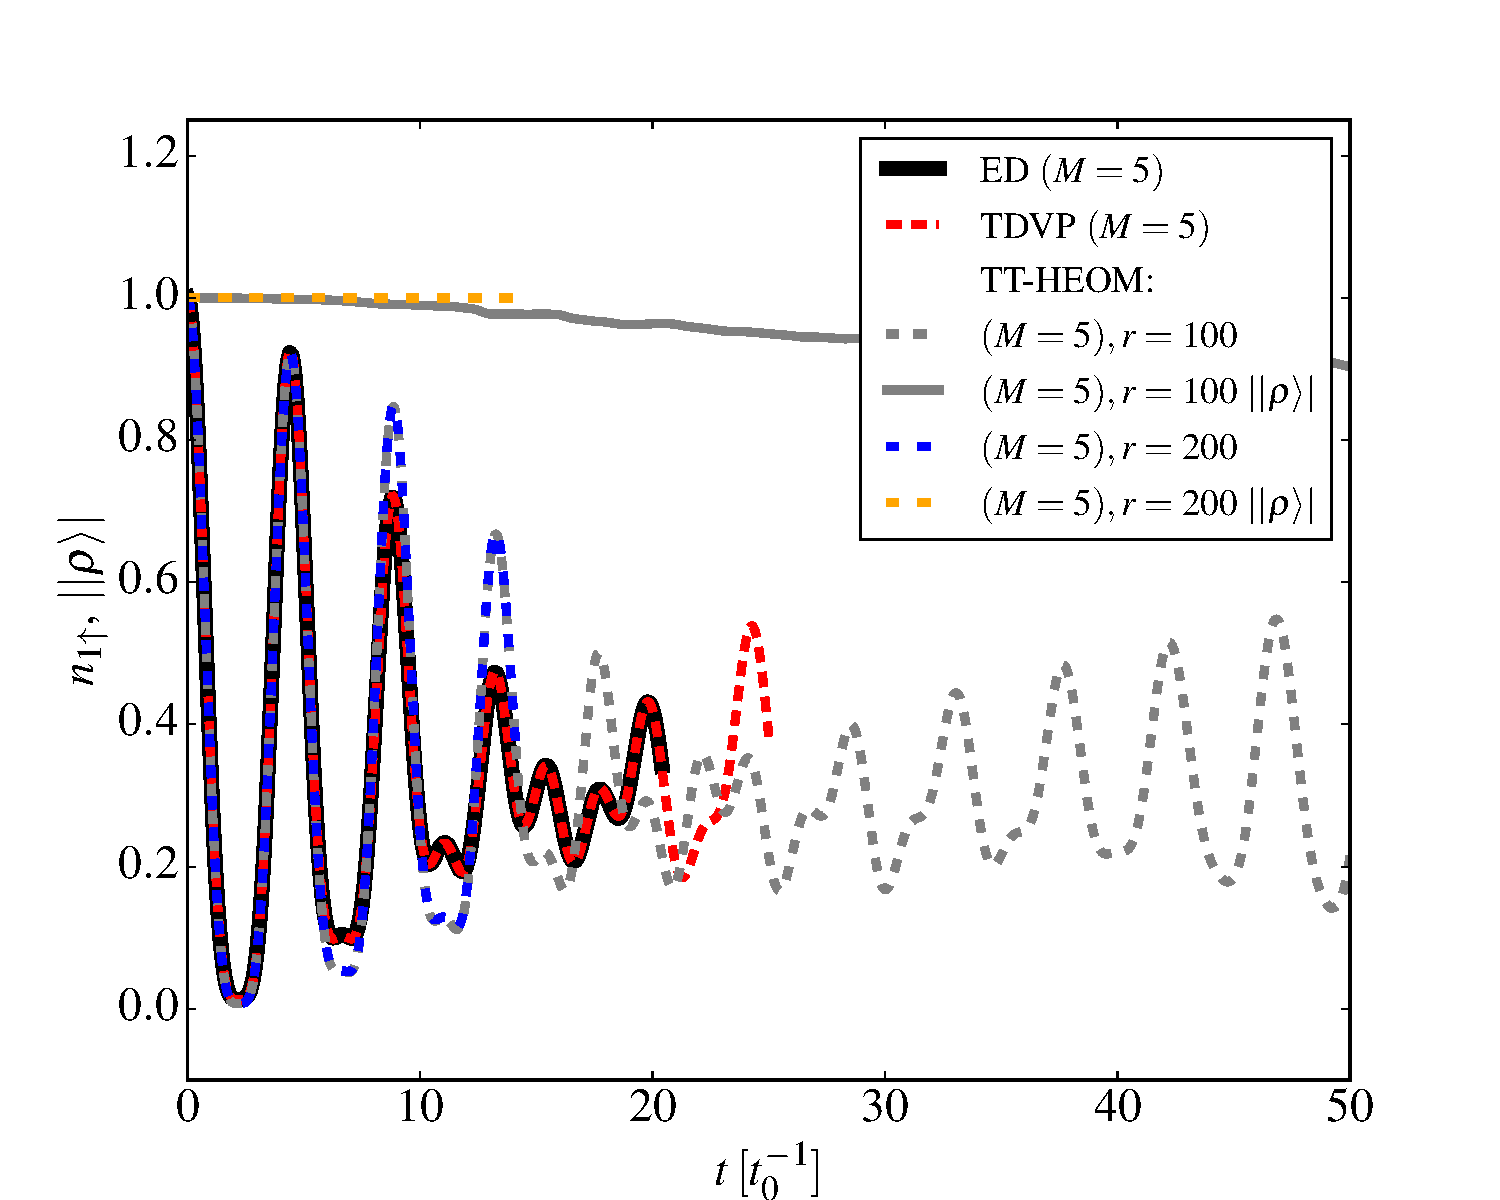
\includegraphics[width=0.705\textwidth]{figs/Comparison_TTHEOM_TDVP_ED_hop+onsite+soc+tph.pdf}
\end{figure}
\subsection{Hopping, SOC, Peierls distortion, and Peierls-SOC}
Parameters: $L=3$, $t_0 = 1$, $\lambda_0 = t_0/40$, $t_1 = 0.1t_0$, $\lambda_1 = 0.1\lambda_0$. This parameter set has been used by Fransson in \cite{fransson2020vibrational}. As it is evident from the comparison of the previous and last-to-previous parameter sets, it is expected that including $\lambda_1$ will not lead to significant changes in the dynamics. Therefore, a comparison here is omitted.
\subsection{Problem statement and possible solution}
The TT-HEOM method converges for purely electronic dynamics when electron-vibrational coupling is omitted. 

In the TT-HEOM method, as implemented currently, a finite electron-vibrational coupling requires a large bond dimension for results to converge as can be seen in the following smaller system with parameters $L=2$, $t_0=1$, $\lambda_0 = t_0/40$, $t_1 = 0.1t_0$, $\lambda_1 = 0.1\lambda_0$, shown below. 
\begin{figure}[!h]
	\centering
	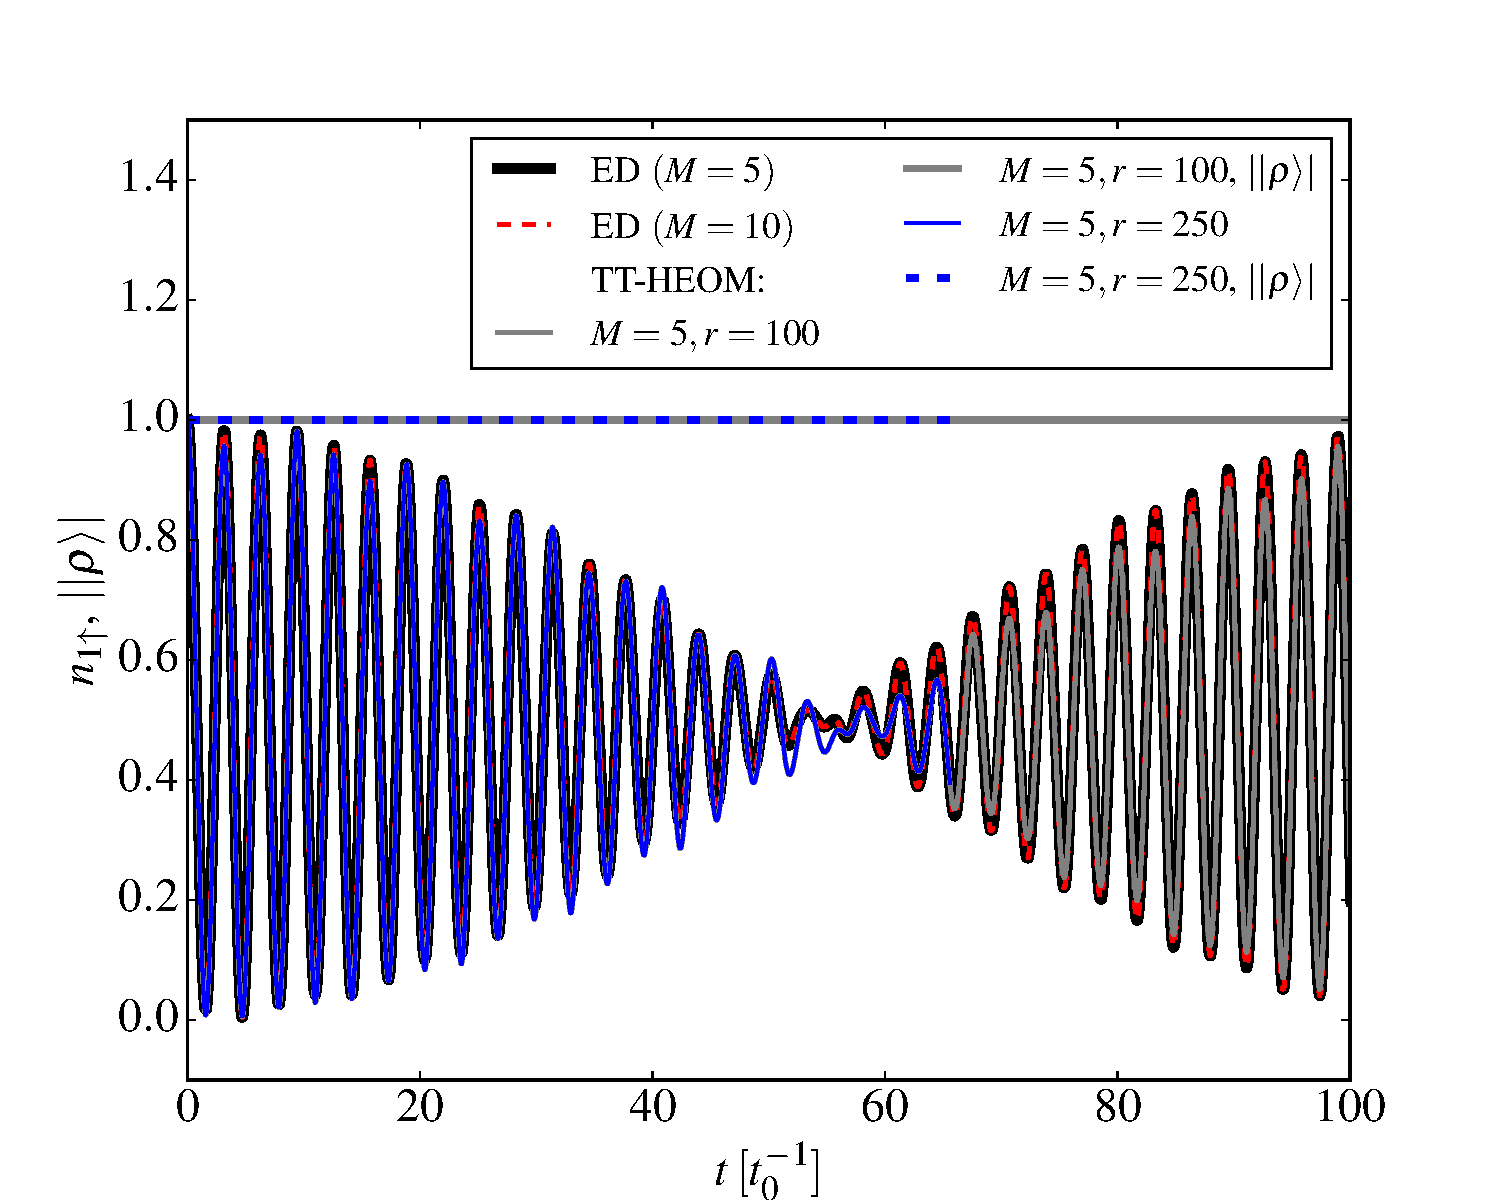
\includegraphics[width=0.8\textwidth]{figs/Comparison_L2_TTHEOM_ED_hop+onsite+soc+tph+socph.pdf}
\end{figure}  \\
It is evident, that the electron-vibrational coupling leads to issues in the TT-HEOM. Currently, an MPS topology is used, in which the state is written as a product over environmental, electronic, and then vibrational core tensors. 
The electronic core tensors are an alternating product of spin up and spin down core tensors. Overall, each site core tensor $i$ is paired with its ancially core tensor $i'$, respectively for the spins $i\uparrow,i'\uparrow,i\downarrow,i'\downarrow$. 
The open source package iTensor (used for obtaining the TDVP results), on the other hand, employs a different MPS topology where the electronic and vibrational core tensors are arranged in an alternating order and the physical dimension of the electronic core tensors is 4 thus including spin. 
None of the above issues were observed in this implementation. Therefore, a change of the MPS topology in the TT-HEOM implementation is promising to yield results which converge with lower bond dimensions.  
\newpage
More precisely, the proposed MPS topology is inspired by the one employed by state-of-the-art MPS-based packages. The current topology is shown below, where $i$ correspond to electronic indices and $j$ to vibrational ones: The physical dimension of the $i$ indices is 2, each core tensor thus describes either up or down spin electrons, while the physical dimension of the $j$ tensors is $M$. 
\begin{figure}[!h]
	\centering
	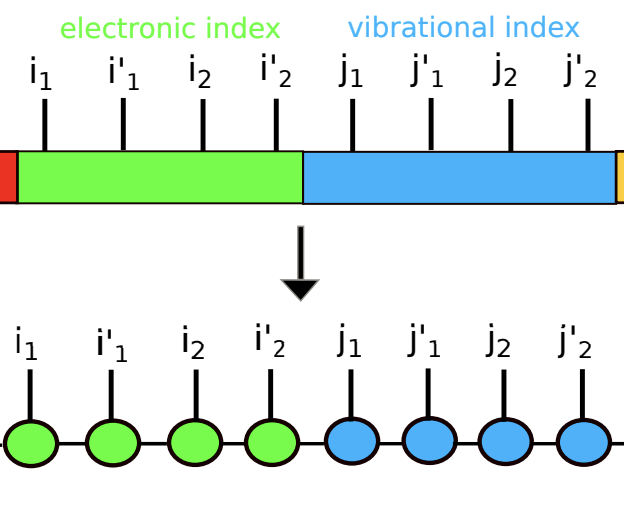
\includegraphics[width=0.3\textwidth]{figs/MPS_topology_old.png}
\end{figure} \\

For solving the convergence issue in an isolated electronic-vibrationally coupled molecule, the proposed topology is shown below. Now, the electronic core tensors $i$ have a physical dimension of 4 instead of 2, the basis is therefore spanned by the states $\vert 00\rangle, \vert 01 \rangle, \vert 10 \rangle$, and $\vert 11\rangle$ where the first state corresponds to electrons with projection $m_s=+1/2$ and second one to electrons with $m_s = -1/2$.
\begin{figure}[!h]
	\centering
	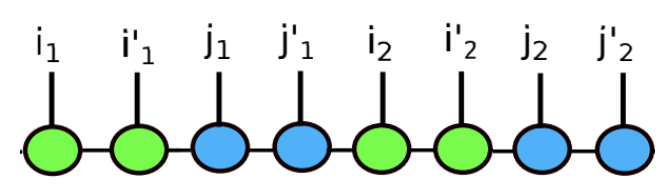
\includegraphics[width=0.3\textwidth]{figs/MPS_topology_new.png}
\end{figure} \\
However, one has to keep in mind that due to the formulation of the TT-HEOM in twin-space and hence addition of auxiliary core tensors, one cannot expect the same efficiency as in the implementation used by iTensor, in which the wavefunction is represented as a MPS. 
\section{Problems in the Dynamics in Open Fransson Model}
\begin{itemize}
	\item Currents at equilibrium using HEOM for non-interacting electrons, even in the absence of vibrations. For systems with SOC, spin currents in equilibrium are known (see, e.g. \cite{rashba2003spin}), but charge currents not.
	\item Spin-current definition as employed before is not applicable anymore, because spin is not conserved due to spin-orbit coupling, see further in Ref. \cite{shi2006proper}
\end{itemize}
\begin{figure}[!h]
	\centering
	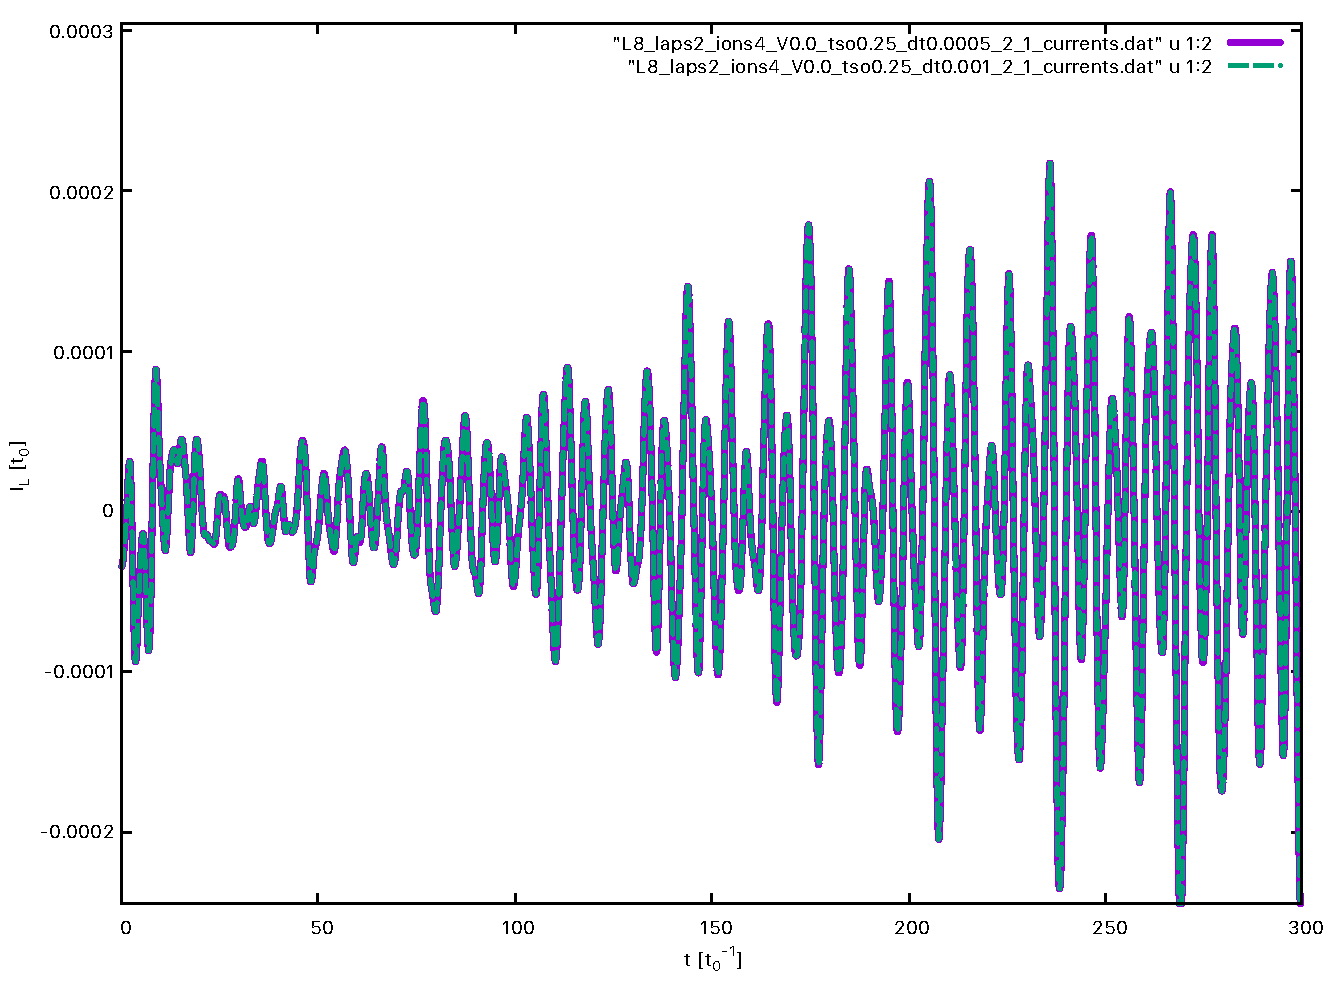
\includegraphics[width=1.0\textwidth]{figs/L8_eqCurrents.pdf}
\end{figure}
%\section{Comparison of Dynamics in Open Molecule}
%\subsection{No vibrations}
%\subsubsection{Hopping}
%Parameters: $L=3$, $t_0 = 1$, $\Gamma = 0.5t_0$, $V=1$, $\beta = 1/0.026$. 
%\subsubsection{Hopping and SOC}
%\subsection{With vibrations}
%\subsubsection{Hopping, SOC and Peierls distortion}
%\subsubsection{Hopping, SOC, Peierls distortion and Peierls SOC}



\printbibliography
\end{document}




